\documentclass[
]{beamer}

\usepackage[czech]{babel}
\usepackage[utf8]{inputenc}
\usepackage[T1]{fontenc}
\usepackage{booktabs}
\usetheme[
  workplace=fi,
]{MU}
\begin{document}

\title[Obhajoba diplomové práce]{Autentizační a autorizační infrastruktura pro videokonferenční prostředí}
\subtitle[Short Presentation Subtitle]{Obhajoba diplomové práce}
\author[L.\,Kotol]{Bc. Lukáš Kotol \\ 433265@mail.muni.cz}
\institute[FI MU]{Fakulta informatiky, Masarykova Univerzita}
\date{\today}
\subject{Presentation Subject}
\keywords{the, presentation, keywords}

\begin{frame}[plain]
\maketitle
\end{frame}

\section[Zadání]{Zadání}

\begin{frame}{Představení zadání}{}
Zadání diplomové práce sestávalo z vytvoření nové \structure{autentizační a autorizační infrastruktury (AAI) pro videokonferenční prostředí}. 
\\
\medskip
Součástí webkonferenčního prostředí jsou služby
\begin{itemize}
  \item meetings.cesnet.cz a
  \item Adobe Connect.
\end{itemize}
\end{frame}

\begin{frame}{Specifikace zadání}
Nová autentizační a autorizační infrastruktura 
\begin{itemize}
  \item bude využívat Proxy IdP v infrastruktuře CESNETu,
  \item bude založena na technologii OpenID Connect a
  \item bude navazovat na stávající AAI. 
\end{itemize}
\end{frame}

\section[Proxy Idp]{Proxy Idp}
\begin{frame}{Proxy IdP infrastruktura}
\begin{itemize}
    \item zajišťuje bezpečný přístup ke službám CESNET eInfrastruktury,
    \item umožňuje delegaci autentizace a autorizace ze služeb 
    \item služby a poskytovatelé identit jsou sdruženy do České akademické federace identit eduID.cz.

\end{itemize}
\end{frame}

\section[OpenID Connect]{OpenID Connect}

\begin{frame}{OpenID Connect}
\framesubtitle{Představení protokolu}
Protokol, umožňující aplikaci verifikovat identitu uživatele na základě autentizace provedené autorizačním serverem.
\\
\medskip
Vlastnosti:
\begin{itemize}
  \item autentizační vrstva nad frameworkem OAuth,
  \item definuje způsob získávání informací o přihlášeném uživateli,
  \item specifikuje REST HTTP API, tzv. Endpointy,
  \item používá JSON.
\end{itemize}
\end{frame}

\begin{frame}{OpenID Connect}
\framesubtitle{Schéma komunikace v protokolu}
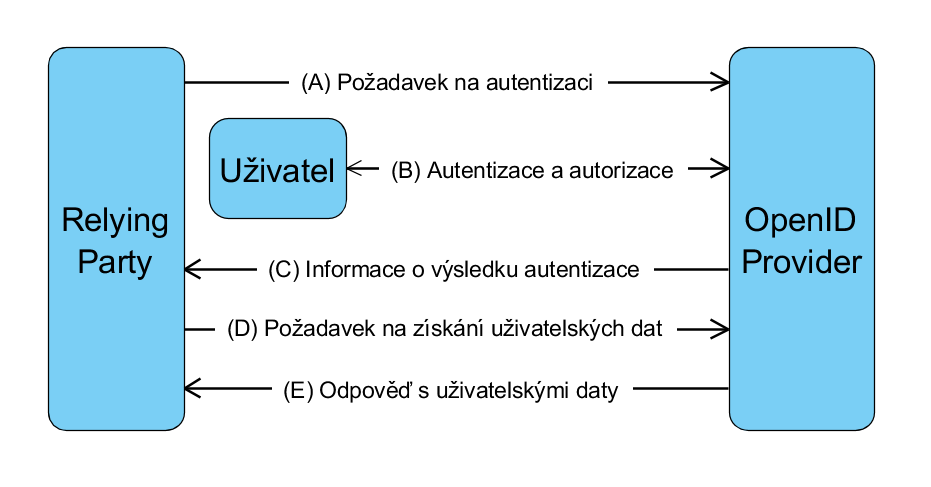
\includegraphics[width=\textwidth]{pics/diplomkaOIDC}
\end{frame}



\begin{frame}{Vypracování DP}

\end{frame}

\begingroup
\setbeamercolor{background canvas}{bg=mubeamer@base}
\begin{frame}[plain]
\vfill
\centering

\includegraphics[width=\textwidth]{institution}
\vfill
\end{frame}
\endgroup

\end{document}
